\def\linkdethi{} %Đường link cần dẫn tới
\anmaQR
%%%%%%%%%%%%%%%%%%%%%%%%
\def\toanlop{12}
\def\thoigian{90}
\def\namhoc{2025 - 2026}
\begin{dethi}
	{Bộ GD\&ĐT}
	{VTED ft KING EDU}
	{TDMT11}
	{Đề thi thử THPTQG 2026}
\end{dethi}
\caulc
\Opensolutionfile{ans}[ans/ansTN-Dung]
%%%=============EX_1=============%%%
\begin{ex}%[1D2N2-3]%[TDMT11]%[Bồ Văn Hậu]
	Cho cấp số cộng $\left(u_n\right)$ có $u_1=1$ và công sai $d=3$. Giá trị của $u_3$ bằng
	\choice
	{\True $7$}
	{$10$}
	{$4$}
	{$9$}
	\loigiai{
		Theo công thức số hạng tổng quát của cấp số cộng, ta có
		\[u_3=u_1+2d=1+2\cdot 3=7.\]
	}
\end{ex}
%%%=============================%%%

%%%=============EX_2=============%%%
\begin{ex}%[1D6H3-2]%[TDMT11]%[Đình Nguyên]
	Tập giá trị của hàm số $y=(8-x)^{\sqrt{3}}$ là
	\choice
	{$(-\infty; 8)$}
	{$(-\infty; +\infty)$}
	{$(8; +\infty)$}
	{\True $(0; +\infty)$}
	\loigiai{
		Hàm số đã cho là hàm số lũy thừa có số mũ $\alpha = \sqrt{3}$ là số không nguyên.\\
		Điều kiện xác định: $8 - x > 0 \Leftrightarrow x < 8$.\\
		Ta có $y = (8 - x)^{\sqrt{3}} > 0$.\\
		Vậy tập giá trị của hàm số là $(0; +\infty)$.
	}
\end{ex}
%%%=============================%%%

%%%=============EX_3=============%%%
\begin{ex}%[1D6N4-3]%[TDMT11]%[Trần Văn Thiện]
	Tập nghiệm của bất phương trình $\log_{0{,}25}\left(x-3\right)\geq -1$ là
	\choice
	{$\left(-\infty;7\right]$}
	{$\left(7;+\infty\right)$}
	{ $\left[7;+\infty\right)$}
	{\True$\left(3;7\right]$}
	\loigiai{
		Điều kiện $x-3>0\Leftrightarrow x>3$.\\
		Khi đó phương trình cho trở thành $ x-3\leq 4\Leftrightarrow x\leq 7$.\\
		Kết hợp điều kiện, bất phương trình cho có tập nghiệm $\left(3;7\right]$.
	}
\end{ex}
%%%=============================%%%

%%%=============EX_4=============%%%
\begin{ex}%[1H8H7-2]%[TDMT11]%[Mui Doan]
	Cho hình chóp tứ giác $S.ABCD$ có đáy là hình vuông cạnh $6$. Cạnh bên $SA$ vuông góc với đáy. Biết góc giữa mặt phẳng $(SBC)$ với đáy $(ABCD)$ bằng $60^\circ$. Thể tích khối chóp $S.ABC$ bằng
	\choice
	{$72\sqrt{6}$}
	{$72\sqrt{3}$}
	{\True $36\sqrt{3}$}
	{$54\sqrt{2}$}
	\loigiai{
		\immini{
			Ta có
			$\heva{&(SBC)\cap (ABCD)=BC\\&AB\perp BC\\&SB\perp BC}\\
			\Rightarrow \left((SBC),(ABCD)\right)=(SB,AB)=\widehat{SBA}=60^\circ$.\\
			Tam giác $SAB$ vuông tại $A$ có
			\[
			\tan 60^\circ=\dfrac{SA}{AB}\Rightarrow SA=AB\cdot \tan 60^\circ=6\sqrt{3}.
			\]
			Diện tích đáy $S_{ABC}=\dfrac{1}{2}\cdot 6^2=18$.\\
			Thể tích khối chóp
			\[
			V_{S.ABC}=\dfrac{1}{3}S_{ABC}\cdot SA
			=\dfrac{1}{3}\cdot18\cdot 6\sqrt{3}
			=36\sqrt{3}.
			\]
		}
		{
			\begin{tikzpicture}[declare function={gocx=90; goc=-150; a=5; b=a/2; h=4;}, scale=0.8, line join=round, line cap=round, >=stealth, font=\footnotesize]
				\path (0,0) coordinate (A)--+(gocx:h) coordinate (S)
				(a,0) coordinate (B)
				(goc:b) coordinate (D)
				+(a,0) coordinate (C);
				
				\path pic [draw,"$60^\circ$",angle eccentricity=1.6, angle radius=.6cm] {angle = S--B--A};
				\path pic[angle radius=3mm,draw] {right angle = S--A--B};
				
				\draw[dashed] (S)--(A) (D)--(A)--(B);
				\draw (S)--(D)--(C)--(S)--(B)--(C)--cycle;
				
				\foreach \x/\goc in {S/90, A/150, B/0, C/-60, D/-180} {
					\filldraw (\x) circle (1pt) node[shift={(\goc:3mm)}]{$\x$};
				}
			\end{tikzpicture}
		}
	}
\end{ex}
%%%=============================%%%

%%%=============EX_5=============%%%
\begin{ex}%[2D1H2-1]%[TDMT11]%[Nguyễn Trí Minh Tuấn]
	Hàm số $y = x^3 - 6x^2 + 1$ đạt cực đại tại
	\choice
	{$x=4$}
	{\True $x=0$}
	{$y=1$}
	{$y=0$}
	\loigiai{
		Ta có $y' = 3x^2-12x = 0 \Leftrightarrow \hoac{&x=0\\&x=4.}$\\
		Bảng biến thiên
		\begin{center}
			
\begin{tikzpicture}
				\tkzTabInit[nocadre=false,lgt=1.2,espcl=2.5,deltacl=0.6]
				{$x$/1,$y'$/1,$y$/2}
				{$-\infty$, $0$, $4$, $+\infty$}
				\tkzTabLine{,+,0,-,0,+,}
				\tkzTabVar{-/$-\infty$ , +/$1$ , -/$-31$ , +/$+\infty$}
			\end{tikzpicture}
		\end{center}
		Vậy hàm số đạt cực đại tại $x=0$.
	}
\end{ex}
%%%=============================%%%

%%%=============EX_6=============%%%
\begin{ex}%[1D5H1-3]%[TDMT11]%[Huynh Quốc Đạt]
	Cho mẫu số liệu ghép nhóm $M$ với bảng tần số ghép nhóm như sau
	\begin{center}
		\begin{tabular}{|c|c|c|c|c|c|c|}
			\hline
			Nhóm & {$[6; 8)$} & {$[8; 10)$} & {$[10; 12)$} & {$[12; 14)$} & {$[14; 16)$} & {$[16; 18)$}\\
			\hline
			Tần số & $5$ & $3$ & $6$ & $4$ & $7$ & $5$ \\
			\hline
		\end{tabular}
	\end{center}
	Hãy xác định số trung bình cộng của mẫu số liệu ghép nhóm $M$ (\textit{làm tròn kết quả đến hàng phần mười}).
	\choice
	{$\overline{x}=14{,}6$}
	{$\overline{x}=12{,}0$}
	{\True $\overline{x}=12{,}3$}
	{$\overline{x}=13{,}1$}
	\loigiai{
		Bảng giá trị đại diện
		\begin{center}
			\begin{tabular}{|c|c|c|c|c|c|c|}
				\hline
				Nhóm & {$[6; 8)$} & {$[8; 10)$} & {$[10; 12)$} & {$[12; 14)$} & {$[14; 16)$} & {$[16; 18)$}\\
				\hline
				Giá trị đại diện & $7$ & $9$ & $11$ & $13$ & $15$ & $17$\\
				\hline
				Số học sinh & $5$ & $3$ & $6$ & $4$ & $7$ & $5$ \\
				\hline
			\end{tabular}
		\end{center}
		Số trung bình của mẫu số liệu ghéo nhóm $M$ là
		\[\overline{x}=\dfrac{7\cdot 5+9\cdot 3+11\cdot 6+13\cdot 4+15\cdot 7+17\cdot 5}{5+3+6+4+7+5}\approx 12{,}3.\]
	}
\end{ex}
%%%=============================%%%

%%%=============EX_7=============%%%
\begin{ex}%[2D1H4-1]%[TDMT11]%[Chu Ha]
	Đồ thị hàm số $y=\dfrac{3x-5}{x+1}$ có số đường tiệm cận song song với trục hoành là
	\choice
	{\True $1$}
	{$2$}
	{$0$}
	{$3$}
	\loigiai{
		Ta có
		$\displaystyle \lim\limits_{x\to\pm\infty}\dfrac{3x-5}{x+1}
		=
		\lim\limits_{x\to\pm\infty}\dfrac{3-\dfrac{5}{x}}{1+\dfrac{1}{x}}
		=3$.\\
		Suy ra đồ thị hàm số có một đường tiệm cận song song với trục hoành là $y=3$.
	}
\end{ex}
%%%=============================%%%

%%%=============EX_8=============%%%
\begin{ex}%[2D4N3-3]%[TDMT11]%[Nguyễn Tấn Linh]
	Cho hình phẳng giới hạn bởi các đường $y = f(x)$, $Ox$, $x=1$, $x=3$ quay quanh trục hoành $Ox$ thì khối tròn xoay thu được có thể tích bằng
	\choice
	{$V = \displaystyle\int\limits_1^3 \left[ f(x) \right]^2 \mathrm{\,d}x$}
	{$V = \pi\displaystyle\int\limits_1^3 \left| f(x) \right| \mathrm{\,d}x$}
	{$V = \displaystyle\int\limits_1^3 \left| f(x) \right| \mathrm{\,d}x$}
	{\True $V = \pi\displaystyle\int\limits_1^3 \left[ f(x) \right]^2 \mathrm{\,d}x$}
	\loigiai{
		Thể tích khối tròn xoay sinh bởi hình phẳng giới hạn bởi đồ thị hàm số $y=f(x)$, trục hoành và hai đường thẳng $x=a$, $x=b$ ($a<b$) khi quay quanh trục $Ox$ được tính bởi công thức
		\[V=\pi\displaystyle\int\limits_a^b \left[ f(x) \right]^2 \mathrm{\,d}x.\]
		Áp dụng với cận từ $1$ đến $3$, ta có công thức đúng là $V = \pi\displaystyle\int\limits_1^3 \left[ f(x) \right]^2 \mathrm{\,d}x$.
	}
\end{ex}
%%%=============================%%%

%%%=============EX_9=============%%%
\begin{ex}%[2D4N1-4]%[TDMT11]%[Lê Phúc]
	Họ nguyên hàm của hàm số $f(x)=2^{3x+1}$ tương ứng là
	\choice
	{$2^{3x+1}+C$}
	{\True $\dfrac{2^{3x+1}}{3\ln 2}+C$}
	{$2^{3x+1}\ln 8+C$}
	{$\dfrac{3\cdot 2^{3x+1}}{\ln 8}+C$}
	\loigiai{
		Áp dụng công thức $\displaystyle\int k^{ax+b} \mathrm{\,d}x=\dfrac{1}{k}\cdot \dfrac{k^{ax+b}}{\ln k}+C$.\\
		Khi đó $\displaystyle\int 2^{3x+1} \mathrm{\,d}x=\dfrac{1}{3}\cdot \dfrac{2^{3x+1}}{\ln 2}+C$.
	}
\end{ex}
%%%=============================%%%

%%%=============EX_10=============%%%
\begin{ex}%[2H5N1-5]%[TDMTD11]%[Phạm Hải Dương]
	Trong không gian $Oxyz$, cho mặt phẳng $(\alpha)\colon x-2y+2z+11=0$ và điểm $A(1;0;3)$. Hãy tính $\mathrm{d}\left(A,(\alpha)\right)$.
	\choice
	{$3$}
	{$4$}
	{$5$}
	{\True $6$}
	\loigiai{
		Khoảng cách từ điểm $A(1;0;3)$ đến mặt phẳng $(\alpha)\colon x-2y+2z+11=0$ được tính theo công thức
		\[\mathrm{d}\left(A,(\alpha)\right)=\dfrac{|1\cdot 1-2\cdot 0+2\cdot 3+11|}{\sqrt{1^2+(-2)^2+2^2}}=\dfrac{|1-0+6+11|}{\sqrt{1+4+4}}=\dfrac{18}{\sqrt{9}}=\dfrac{18}{3}=6.\]
		Vậy $\mathrm{d}\left(A,(\alpha)\right)=6$.
	}
\end{ex}
%%%=============================%%%

%%%=============EX_11=============%%%
\begin{ex}%[2H2V1-2]%[TDM21]%[Huỳnh Trí Thiện]
	Cho hình lăng trụ $ABC.A'B'C'$ có $G$ là trọng tâm của tam giác $A'B'C'$. Hỏi khi đó $\overrightarrow{AA'} + \overrightarrow{AB'} - 2\cdot\overrightarrow{AC'}$ bằng với vectơ nào dưới đây?
	\choice
	{$3\cdot\overrightarrow{AC'}$}
	{\True $3\cdot\overrightarrow{C'G}$}
	{$3\cdot\overrightarrow{C'A}$}
	{$\overrightarrow{AC'}$}
	\loigiai{
		\immini{Vì $G$ là trọng tâm của tam giác $A'B'C'$, nên với điểm $A$ bất kỳ ta có đẳng thức
			\[ \overrightarrow{AA'} + \overrightarrow{AB'} + \overrightarrow{AC'} = 3\cdot\overrightarrow{AG}. \]
			Biến đổi biểu thức vectơ của đề bài như sau
			\allowdisplaybreaks
			\begin{align*}
				\overrightarrow{AA'} + \overrightarrow{AB'} - 2\cdot\overrightarrow{AC'} &= \left( \overrightarrow{AA'} + \overrightarrow{AB'} + \overrightarrow{AC'} \right) - 3\cdot\overrightarrow{AC'} \\
				&= 3\cdot\overrightarrow{AG} - 3\cdot\overrightarrow{AC'} \\
				&= 3\cdot\left( \overrightarrow{AG} - \overrightarrow{AC'} \right) \\
				&= 3\cdot\overrightarrow{C'G}.
			\end{align*}
			Vậy $\overrightarrow{AA'} + \overrightarrow{AB'} - 2\cdot\overrightarrow{AC'} = 3\cdot\overrightarrow{C'G}$.
		}{
			\begin{tikzpicture}[declare function={ac=4; ab=2; h=4; gocA=50;}, scale=0.8, font=\footnotesize, line join=round, line cap=round, >=stealth]
				\coordinate[label=left:$B$] (A) at (0,0);
				\coordinate[label=right:$C$] (C) at (ac,0);
				\coordinate[label=below left:$A$] (B) at (-gocA:ab);
				\coordinate[label=left:$B'$] (A') at ($(A)+(60:h)$);
				\coordinate[label=below right:$A'$] (B') at ($(B)-(A)+(A')$);
				\coordinate[label=right:$C'$] (C') at ($(C)-(A)+(A')$);
				
				\draw (A')--(A)--(B)--(C)--(C')--(A')--(B')--(C')--(B) (A')--(B');
				\draw[dashed] (A)--(C);
				
				\coordinate (M) at ($(B')!0.5!(C')$);
				\coordinate[label=above:$G$] (G) at ($(A')!2/3!(M)$);
				
				\draw[thin] (A')--(M); 
				\draw[->, red, thick] (C')--(G);
				\draw[->, blue, thick] (B)--(A');
				\draw[->, blue, thick] (B)--(C');
				\draw[->, blue, thick] (B)--(B');
				
				\foreach \diem in {A,B,C,A',B',C',G} \filldraw (\diem) circle (1pt);
				\filldraw (M) circle (0.8pt);
			\end{tikzpicture}
	}}
\end{ex}
%%%=============================%%%

%%%=============EX_12=============%%%
\begin{ex}%[2H5H3-3]%[TDMT11]%[Nguyễn Sơn Thành]
	Trong không gian $Oxyz$, phương trình mặt cầu $(S)$ có tâm $I$ nằm trên tia $Oy$ và đi qua $O$, cách gốc $O$ một đoạn bằng $4$ là
	\choice
	{\True $x^2 + (y - 4)^2 + z^2 = 16$}
	{$x^2 + (y + 4)^2 + z^2 = 16$}
	{$x^2 + (y - 4)^2 + z^2 = 4$}
	{$(x - 4)^2 + y^2 + (z - 4)^2 = 16$}
	\loigiai{
		\begin{itemize}
			\item Vì tâm $I$ nằm trên tia $Oy$ và cách gốc tọa độ $O$ một khoảng bằng $4$, nên tọa độ của tâm $I$ là $I(0; 4; 0)$.
			\item Mặt cầu $(S)$ đi qua gốc tọa độ $O$, do đó bán kính $R$ của mặt cầu là\\ $R = OI = \sqrt{(0-0)^2 + (4-0)^2 + (0-0)^2} = 4$.
			\item Phương trình mặt cầu $(S)$ có tâm $I(0; 4; 0)$ và bán kính $R=4$ là $x^2 + (y - 4)^2 + z^2 = 16$.
		\end{itemize}
	}
\end{ex}
%%%=============================%%%
\Closesolutionfile{ans}
\cauds
\Opensolutionfile{ans}[ans/ansTN-DungSai]
%%%=============EX_13=============%%%
\begin{ex}%[2D4H3-1]%[TDMT11]%[Dương Công Tạo]
	Cho hàm số $y=f(x)=x^3-6x^2+9x$ có đồ thị $(C)$.
	\choiceTF[t]
	{\True Tất cả các nguyên hàm của $f(x)$ đều có ít số điểm cực trị hơn $f(x)$}
	{\True Hàm số $f(x)$ nghịch biến trên khoảng $(1; 3)$}
	{\True Hai điểm cực trị của $(C)$ cách nhau một khoảng bằng $2\sqrt{5}$}
	{Diện tích hình phẳng giới hạn bởi $(C)$ và trục hoành bằng $4$ \textit{(làm tròn kết quả đến hàng đơn vị)}}
	\loigiai{
		Xét hàm số $f(x)=x^3-6x^2+9x$.\\
		Tập xác định $\mathscr{D}=\mathbb{R}$.\\
		Ta có $f'(x)=3x^2-12x+9$, $f'(x)=0\Leftrightarrow \hoac{&x=3\\&x=1.}$\\
		Bảng biến thiên
		\begin{center}
			
\begin{tikzpicture}[>=stealth]
				\tkzTabInit[nocadre=false,lgt=1.5,espcl=2,deltacl=0.6]{$x$/.7 ,$f'(x)$/.7,$f(x)$/2}
				{$-\infty$ , $1$ , $3$ , $+\infty$}
				\tkzTabLine{ , + , 0 , - , 0 , + , }
				\tkzTabVar{-/$-\infty$ , +/$4$ , -/$0$ , +/$+\infty$}
			\end{tikzpicture}
		\end{center}
		Dựa vào bảng biến thiên, ta thấy hàm số đạt
		\begin{itemize}
			\item cực đại tại điểm $x=1\Rightarrow y_{\text{CĐ}}=4$;
			\item cực tiểu tại $x=3\Rightarrow y_{\text{CT}}=0$.
		\end{itemize}
		\begin{itemchoice}
			\itemch Gọi $F(x)$ là nguyên hàm số $f(x)$.\\
			Ta có $F'(x)=f(x)$, $F'(x)=f(x)=x\left(x^2-6x+9\right)=x(x-3)^2$, $F'(x)=0\Leftrightarrow\hoac{&x=0\\&x=3.}$\\
			Bảng biến thiên
			\begin{center}
				
\begin{tikzpicture}[>=stealth]
					\tkzTabInit[nocadre=false,lgt=1.5,espcl=2,deltacl=0.6]{$x$/.7 ,$F'(x)$/.7,$F(x)$/2}
					{$-\infty$ , $0$ , $3$ , $+\infty$}
					\tkzTabLine{ , - , 0 , + , 0 , + , }
					\tkzTabVar{+/$+\infty$ , -/$0$ , R , +/$+\infty$}
				\end{tikzpicture}
			\end{center}
			Dựa vào bảng biến thiên, ta thấy hàm số đạt đạt cực tiểu tại $x=0$.\\
			Vậy $F(x)$ có ít số điểm cực trị hơn $f(x)$.
			\itemch Dựa vào bảng biến thiên, ta thấy hàm số $f(x)$ nghịch biến trên khoảng $(1;3)$.
			\itemch Gọi $A(1;4)$, $B(3;0)$ lần lượt là hai điểm cực trị của đồ thị $(C)$.\\
			Ta có $AB=\sqrt{(3-1)^2+(0-4)^2}=2\sqrt{5}$.
			\itemch Ta có $f(x)=x\left(x^2-6x+9\right)=x(x-3)^2\Rightarrow f(x)=0\Leftrightarrow \hoac{&x=0\\&x=3.}$\\
			Vì $f(x)\geq 0$, $\forall x\in[0;3]$ nên diện tích hình phẳng giới hạn bởi $(C)$ và trục hoành là 
			\[S=\displaystyle\int\limits_0^3{\left(x^3-6x^2+9x\right)}\mathrm{\,d}x=\left.\left(\dfrac{x^4}{4}-2x^3+\dfrac{9x^2}{2}\right)\right|_0^3=\dfrac{27}{4}=6{,}75\approx 7.\]
			Vậy, diện tích hình phẳng giới hạn bởi $(C)$ và trục hoành bằng $7$.
		\end{itemchoice}
	}
\end{ex}
%%%=============================%%%

%%%=============EX_14=============%%%
\begin{ex}%[2H5V2-8]%[TDMT11]%[Vũ Hồng Toàn]
	Trong không gian $Oxyz$ có đơn vị dài trên mỗi trục là kilômét, mặt đất là mặt phẳng $(Oxy)$. Một chiếc máy bay đang ở vị trí $A(4;-3{,}5;1)$ và sẽ hạ cánh ở vị trí $B(4;8{,}5;0)$ trên đường băng. Trên đoạn $AB$ thì tốc độ của máy bay không đổi bằng $150\mathrm{\,km/h}$. Một đám mây mỏng được mô phỏng bởi mặt phẳng $(\alpha)$ đi qua ba điểm $M(8;0;0)$, $N(0;-12;0)$, $P(0;0;1)$.
	\begin{center}
		\begin{tikzpicture}[line join=round, line cap=round, >=stealth, font=\footnotesize, scale=0.5]
			\path 
			(0,0) coordinate (O)
			(-9,0) coordinate (N)
			($(O)!1!40:(N)$) coordinate (M)
			(0,0.9) coordinate (P)
			($(O)!1.2!(M)$) coordinate (x)
			(-5,0.8) coordinate (A)
			(4,-1.5) coordinate (B)
			($(A)!2.1cm!(B)$) coordinate (C)
			(intersection of A--B and O--M) coordinate (B1);
			
			\draw[line width=0.3mm,red] (A)--(C) (B1)--(B);
			\draw[line width=0.3mm,red,dashed] (C)--(B1);
			\draw[->,>=stealth,line width=0.3mm,blue] (0,0)--(x) node[right=0.2cm]{$x$};
			\draw[->,>=stealth,line width=0.3mm,blue] (-10,0)--(-9,0) (0,0) node[above right]{$O$}--(7,0) node[below]{$y$};
			\draw[line width=0.3mm,blue,dashed] (-9,0)--(0,0);
			\draw[->,>=stealth,line width=0.3mm,blue] (0,0)--(0,3) node[left]{$z$};
			\draw[line width=0.3mm,blue] (N)--(P)--(M) (N)--(M);
			
			\foreach \x/\gm in {N/90, P/140} {
				\filldraw (\x) circle (1pt) node[shift={(\gm:5mm)}, blue]{$\x$};
			}
			
			\node[below left,blue] at (N) {$-9$};
			\node[blue,above right] at (P) {$0{,}9$};
			\filldraw (M) circle (1pt) node[blue,right=0.1cm]{$9$} node[blue,left=0.1cm]{$M$};
			\filldraw[red] (C) circle (3pt) node[below=0.2cm,blue]{\scriptsize $C$} 
			(A) circle (3pt) node[above left,blue]{$A$} 
			(B) circle (3pt) node[below,blue]{$B$};
		\end{tikzpicture}
	\end{center}
	\choiceTF[t]
	{\True Khoảng thời gian máy bay đi từ $A$ đến $B$ là $289$ giây \textit{(làm tròn kết quả đến hàng đơn vị)}}
	{\True Đám mây nằm trên mặt phẳng có phương trình tổng quát $12x-8y+96z-96=0$}
	{\True Trong quá trình hạ cánh máy bay sẽ xuyên qua đám mây}
	{\True Khi gặp đám mây thì máy bay đang ở độ cao là $604\mathrm{\,m}$ \textit{(tính theo đơn vị mét và làm tròn kết quả đến hàng đơn vị)}}
	\loigiai{
		\begin{itemchoice}
			\itemch Độ dài đoạn $AB = \sqrt{0^2 + 12^2 + (-1)^2} = \sqrt{145}\mathrm{\,(km)}$.\\
			Do đó, khoảng thời gian máy bay đi từ $A$ đến $B$ là
			\[t=\dfrac{\sqrt{145}}{150}\text{ (giờ)}=\dfrac{\sqrt{145}}{150}\cdot 3\,600\approx 289\text{ (giây)}.\]
			\itemch Mặt phẳng $(\alpha)$ qua $M(8;0;0)$, $N(0;-12;0)$, $P(0;0;1)$ nên có phương trình
			\[\dfrac{x}{8}+\dfrac{y}{-12}+\dfrac{z}{1}=1\Leftrightarrow 12x-8y+96z-96=0.\]
			\itemch Đoạn $AB$ đi qua $A(4;-3{,}5;1)$ và có một vectơ chỉ phương là $\overrightarrow{AB}=(0;12;-1)$ nên có phương trình
			$\heva{&x=4\\&y=-3{,}5+12t\\&z=1-t},\; (t\in[0;1])$.\\
			Gọi $C=AB\cap (\alpha)\Rightarrow C(4;-3{,}5+12t;1-t)$.\\
			Thay tọa độ điểm $C$ vào phương trình mặt phẳng $(\alpha)\colon 12x-8y+96z-96=0\Leftrightarrow (\alpha)\colon 3x - 2y + 24z - 24=0$ ta được
			\allowdisplaybreaks
			\begin{align*}
				& 3\cdot 4 - 2(-3{,}5+12t) + 24\cdot (1-t) - 24=0\\
				\Leftrightarrow & 19-48t=0\Leftrightarrow t=\dfrac{19}{48}.
			\end{align*}
			Vì $t=\dfrac{19}{48}\in [0;1]$ do đó đường thẳng $AB$ cắt mặt phẳng $(\alpha)$ tức là trong quá trình hạ cánh máy bay sẽ xuyên qua đám mây.
			\itemch Từ kết quả câu trên suy ra $C\left(4; \dfrac{5}{4}; \dfrac{29}{48}\right)$.\\
			Độ cao của máy bay khi gặp đám mây là
			\[\mathrm{d}(C,(Oxy))=\dfrac{29}{48}\text{ (km)}=\dfrac{29}{48}\cdot 1\,000\approx 604\mathrm{\,(m)}.\]
		\end{itemchoice}
	}
\end{ex}
%%%=============================%%%

%%%=============EX_15=============%%%
\begin{ex}%[2D4V3-5]%[TDM32]%[Nguyễn Văn Sang]
	\immini[thm]{Hình vẽ bên dưới cho biết hình phẳng $(H)$ giới hạn bởi các cạnh $AB=CD=10\mathrm{\,cm}$, $BC=52\mathrm{\,cm}$, cung tròn $AG$ có tâm nằm trên cạnh $BC$, cung parabol $GD$. Biết độ dài $AG=40\mathrm{\,cm}$ và điểm trên cung parabol $GD$ gần với cạnh $BC$ nhất một khoảng bằng $5\mathrm{\,cm}$. Tiến hành gắn hệ trục tọa độ $Oxy$ vào hình $(H)$, sao cho}{
		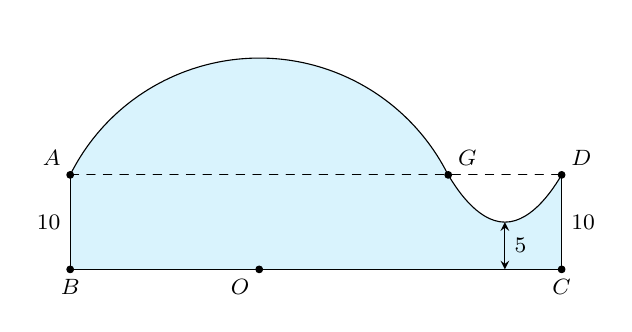
\begin{tikzpicture}[declare function={R=2.236;}, scale=1.2, >=stealth, font=\footnotesize, line join=round, line cap=round]
			\coordinate (O) at (0,0);
			\coordinate (B) at (-2,0);
			\coordinate (C) at (3.2,0);
			\coordinate (A) at (-2,1);
			\coordinate (D) at (3.2,1);
			\coordinate (G) at (2,1);
			\coordinate (V) at (2.6,0.5);
			
			\fill[cyan!15] (B) -- (A) arc ({180-atan(0.5)}:{atan(0.5)}:R) -- (G) parabola bend (V) (D) -- (C) -- cycle;
			
			\draw (B) -- (C) (B) -- (A) (C) -- (D);
			\draw (A) arc ({180-atan(0.5)}:{atan(0.5)}:R);
			\draw (G) parabola bend (V) (D);
			
			\foreach \p in {O,A,B,C,D,G} { \filldraw (\p) circle (1pt); }
			
			\node[below left] at (O) {$O$};
			\node[below] at (B) {$B$}; 
			\node[below] at (C) {$C$};
			\node[above left] at (A) {$A$}; 
			\node[above right] at (G) {$G$}; 
			\node[above right] at (D) {$D$};
			
			\draw[dashed] (A) -- (G) -- (D);
			\draw[<->] (2.6,0.5) -- (2.6,0) node[midway, right]{$5$};
			
			\draw (A) -- (B) node[midway, left]{$10$};
			\draw (C) -- (D) node[midway, right]{$10$};
	\end{tikzpicture}}
	\noindent
	gốc tọa độ $O$ là tâm của cung tròn, trục $Ox$ hướng theo vectơ $\overrightarrow{BC}$, trục $Oy$ hướng theo vectơ $\overrightarrow{BA}$, đơn vị trên mỗi trục tính theo centimet.
	\choiceTF[t]
	{\True $B(-20;0)$, $D(32;10)$}
	{Phương trình cung tròn $AG$ là $y = \sqrt{400 - x^2}$}
	{\True Diện tích của $(H)$ bằng $834\mathrm{\,cm}^2$ \textit{(làm tròn kết quả đến hàng đơn vị)}}
	{\True Thể tích khối tròn xoay thu được khi cho $(H)$ quay quanh trục $Ox$ bằng $47\,836\mathrm{\,cm}^3$ \textit{(làm tròn kết quả đến hàng đơn vị)}}
	\loigiai{
		\immini{
			Chọn hệ trục tọa độ $Oxy$ như hình vẽ, gốc $O$ trùng với tâm cung tròn, trục $Ox$ cùng phương với $\overrightarrow{BC}$, trục $Oy$ vuông góc với $Ox$.
			\begin{itemize}
				\item Do tính chất đối xứng của cung tròn tâm $O$ qua trục tung $Oy$, và $AG=40$ nên $x_G = 20, x_A = -20$.
				Vì $AB=10 \Rightarrow y_A = y_G = 10$. Vậy toạ độ hai điểm là $A(-20; 10)$ và $G(20; 10)$.
				\item Điểm $B$ là hình chiếu của $A$ lên $Ox \Rightarrow B(-20; 0)$.
			\end{itemize}
		}{
			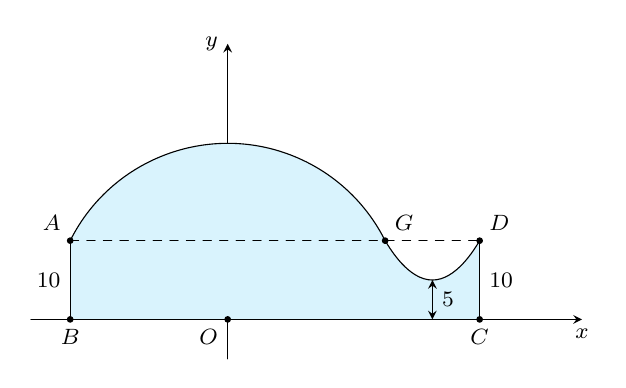
\begin{tikzpicture}[declare function={R=2.236;}, scale=1, >=stealth, font=\footnotesize, line join=round, line cap=round]
				\draw[->] (-2.5,0) -- (4.5,0) node[below]{$x$};
				\draw[->] (0,-0.5) -- (0,3.5) node[left]{$y$};
				
				\coordinate (O) at (0,0);
				\coordinate (B) at (-2,0);
				\coordinate (C) at (3.2,0);
				\coordinate (A) at (-2,1);
				\coordinate (D) at (3.2,1);
				\coordinate (G) at (2,1);
				\coordinate (V) at (2.6,0.5);
				
				\fill[cyan!15] (B) -- (A) arc ({180-atan(0.5)}:{atan(0.5)}:R) -- (G) parabola bend (V) (D) -- (C) -- cycle;
				
				\draw (B) -- (C) (B) -- (A) (C) -- (D);
				\draw (A) arc ({180-atan(0.5)}:{atan(0.5)}:R);
				\draw (G) parabola bend (V) (D);
				
				\foreach \p in {O,A,B,C,D,G} { \filldraw (\p) circle (1pt); }
				
				\node[below left] at (O) {$O$};
				\node[below] at (B) {$B$}; 
				\node[below] at (C) {$C$};
				\node[above left] at (A) {$A$}; 
				\node[above right] at (G) {$G$}; 
				\node[above right] at (D) {$D$};
				
				\draw[dashed] (A) -- (G) -- (D);
				\draw[<->] (2.6,0.5) -- (2.6,0) node[midway, right]{$5$};
				
				\draw (A) -- (B) node[midway, left]{$10$};
				\draw (C) -- (D) node[midway, right]{$10$};
		\end{tikzpicture}}
		\begin{itemize}
			\item Cạnh $BC=52$, suy ra $x_C = x_B + 52 = -20 + 52 = 32 \Rightarrow C(32; 0)$.
			\item $CD \perp BC$ và $CD=10 \Rightarrow D(32; 10)$.
			\item Bán kính cung tròn là $R = OA = \sqrt{(-20)^2 + 10^2} = \sqrt{500}$.
			\item Gọi $V$ là đỉnh của parabol, ta có hoành độ $x_V$ là trung điểm của đoạn hình chiếu của dây $GD$ lên $Ox$
			\[x_V = \dfrac{x_G + x_D}{2} = \dfrac{20+32}{2} = 26.\]
			Tung độ đỉnh $V$ cách đáy $BC$ một khoảng bằng $5 \Rightarrow y_V = 5$. Vậy $V(26; 5)$.
			\item Parabol có đỉnh $V(26;5)$ nên có phương trình dạng $y=a(x-26)^2+5$. Parabol đi qua $G(20;10)$ nên $10=a(20-26)^2+5 \Leftrightarrow a=\dfrac{5}{36}$. Vậy phương trình parabol là $y=\dfrac{5}{36}(x-26)^2+5$.
		\end{itemize}
		\begin{itemchoice}
			\itemch Từ tọa độ đã tìm được $B(-20; 0)$ và $D(32; 10)$.
			\itemch Phương trình đường tròn tâm $O$ bán kính $R=\sqrt{500}$ là $x^2 + y^2 = 500 \Rightarrow y = \sqrt{500 - x^2}$ (vì $y \ge 0$).
			\itemch Diện tích hình phẳng $(H)$
			\[S = \displaystyle\int\limits_{-20}^{20} \sqrt{500-x^2} \mathrm{\,d}x + \displaystyle\int\limits_{20}^{32} \left[ \dfrac{5}{36}(x-26)^2 + 5 \right] \mathrm{\,d}x\approx 833{,}53\approx 834.\]
			\itemch Thể tích khối tròn xoay
			\[V = \pi \displaystyle\int\limits_{-20}^{20} (500-x^2) \mathrm{\,d}x + \pi \displaystyle\int\limits_{20}^{32} \left[ \dfrac{5}{36}(x-26)^2 + 5 \right]^2 \mathrm{\,d}x\approx 47\,835{,}98\approx 47\,836.\]
		\end{itemchoice}
	}
\end{ex}
%%%=============================%%%

%%%=============EX_16=============%%%
\begin{ex}%[2D6V2-4]%[TDMT11]%[Văn Minh Thoại]
	Khối $12$ của một trường THPT được thống kê và thấy có $60\%$ học sinh thích khối $A$, $30\%$ thích khối $B$. Giả sử mỗi học sinh chỉ được thích duy nhất một khối và khi thống kê chỉ quan tâm tới ba khối $A$, $B$, $C$. Biết rằng trong các bạn học sinh nam có $75\%$ là thích khối $A$, $20\%$ thích khối $B$ còn trong các bạn nữ chỉ có $35\%$ thích khối $A$. Chọn ngẫu nhiên một học sinh từ khối $12$ của trường này.
	\choiceTF[t]
	{\True Xác suất để chọn được học sinh thích khối $C$ là $0{,}1$}
	{\True Xác suất chọn được học sinh thích khối $A$ biết học sinh là nữ, bằng $0{,}35$}
	{Xác suất để chọn được học sinh nữ là $0{,}6$}
	{Xác suất chọn được học sinh nam, biết học sinh này thích khối $A$, bằng $\dfrac{8}{11}$}
	\loigiai{
		Gọi $H$ là biến cố học sinh được chọn là nam, $\overline{H}$ là biến cố học sinh được chọn là nữ.\\
		Gọi $A$, $B$, $C$ lần lượt là các biến cố học sinh thích khối $A$, khối $B$, khối $C$.
		\begin{itemchoice}
			\itemch Theo giả thiết, mỗi học sinh chỉ thích duy nhất một khối trong ba khối $A$, $B$, $C$ nên các biến cố $A$, $B$, $C$ là xung khắc và tạo thành một hệ đầy đủ.\\
			Do đó $\mathrm{P}(C)=1-\mathrm{P}(A)-\mathrm{P}(B)=1-0{,}6-0{,}3=0{,}1$.
			\itemch Xác suất chọn được học sinh thích khối $A$ biết học sinh là nữ chính là xác suất có điều kiện $\mathrm{P}\left(A\mid\overline{H}\right)$. \\
			Theo giả thiết, trong các bạn nữ có $35\%$ thích khối $A$, nên $\mathrm{P}\left(A\mid \overline{H}\right)=35\%=0{,}35$.
			\itemch Áp dụng công thức xác suất toàn phần cho biến cố $A$, ta được
			\[\mathrm{P}(A)=\mathrm{P}(H)\cdot \mathrm{P}(A\mid H)+\mathrm{P}\left(\overline{H}\right)\cdot \mathrm{P}\left(A\mid\overline{H}\right).\]
			Đặt $\mathrm{P}(H)=x$, $(0<x<1)\Rightarrow \mathrm{P}\left(\overline{H}\right)=1-x$.\\
			Theo giả thiết có $\mathrm{P}(A)=0{,}6$; $\mathrm{P}(A\mid H)=0{,}75$; $\mathrm{P}\left(A\mid\overline{H}\right)=0{,}35$, khi đó
			\allowdisplaybreaks
			\begin{align*}
				0{,}6 &= x\cdot 0{,}75+(1-x)\cdot 0{,}35\\
				\Leftrightarrow 0{,}6 &= 0{,}75x+0{,}35-0{,}35x\\
				\Leftrightarrow 0{,}4x &= 0{,}25\\
				\Leftrightarrow x &= 0{,}625.
			\end{align*}
			Vậy $\mathrm{P}(H)=0{,}625$ và xác suất chọn được học sinh nữ là $\mathrm{P}\left(\overline{H}\right)=1-0{,}625=0{,}375$.
			\itemch Xác suất chọn được học sinh nam, biết học sinh này thích khối $A$ là
			\[\mathrm{P}(H\mid A)=\dfrac{\mathrm{P}(H\cap A)}{\mathrm{P}(A)}=\dfrac{\mathrm{P}(H)\cdot \mathrm{P}(A\mid H)}{\mathrm{P}(A)}=\dfrac{0{,}625\cdot 0{,}75}{0{,}6}=\dfrac{25}{32}.\]
		\end{itemchoice}
	}
\end{ex}
%%%=============================%%%
\Closesolutionfile{ans}

\caukq 
\Opensolutionfile{ans}[ans/ansTN-DienKhuyet]
%%%=============EX_17=============%%%
\begin{ex}%[TDMT11]%[Lương Pho]%[1H8V7-8]
	Cho hình lăng trụ đứng $ABC.A'B'C'$ có độ dài các cạnh đáy $AB = 5$, $BC = 6$, $CA = 7$. Biết $\mathrm{d}\left(A',\left(AB'C'\right)\right) = 3$. Hãy tính thể tích của lăng trụ $ABC.A'B'C'$ (\textit{làm tròn kết quả đến hàng đơn vị}).
	\par
	\shortans[0]{56}
	\loigiai{
		\immini{
			Gọi $\alpha = \widehat{A'C'B'}$. Áp dụng định lí côsin trong tam giác $A'B'C'$, ta có:
			\[ \cos \alpha = \dfrac{A'C'^2 + B'C'^2 - A'B'^2}{2 \cdot A'C' \cdot B'C'} = \dfrac{7^2 + 6^2 - 5^2}{2 \cdot 7 \cdot 6} = \dfrac{5}{7}. \]
			Suy ra $\sin \alpha = \sqrt{1 - \left(\dfrac{5}{7}\right)^2} = \sqrt{\dfrac{24}{49}} = \dfrac{2\sqrt{6}}{7}$.\\
			Kẻ $A'I \perp B'C'$ tại $I$. Khi đó khoảng cách từ $A'$ đến $B'C'$ là:
			\[ x = A'I = A'C' \cdot \sin \alpha = 7 \cdot \dfrac{2\sqrt{6}}{7} = 2\sqrt{6}. \]
			Gọi $h = AA'$ là chiều cao của lăng trụ. Vì $AA' \perp (A'B'C')$ nên $AA' \perp A'I$. Kẻ $A'H \perp AI$ tại $H$, ta chứng minh được $A'H \perp (AB'C')$.\\
			Theo giả thiết, $\mathrm{d}\left(A', (AB'C')\right) = A'H = 3$. \\
			Xét tam giác vuông $AA'I$ với đường cao $A'H$, ta có:
			\[ \dfrac{1}{A'H^2} = \dfrac{1}{h^2} + \dfrac{1}{x^2} \Leftrightarrow \dfrac{1}{3^2} = \dfrac{1}{h^2} + \dfrac{1}{(2\sqrt{6})^2} \Rightarrow \dfrac{1}{h^2} = \dfrac{1}{9} - \dfrac{1}{24} = \dfrac{5}{72}. \]
			Suy ra $h = \sqrt{\dfrac{72}{5}} = \dfrac{6\sqrt{10}}{5}$.\\
			Thể tích của khối lăng trụ $ABC.A'B'C'$ là:
			\begin{eqnarray*}
				V_{ABC.A'B'C'} &=& S_{\triangle A'B'C'} \cdot h = \left(\dfrac{1}{2} \cdot A'C' \cdot B'C' \cdot \sin \alpha\right) \cdot h \\
				&=& \dfrac{1}{2} \cdot 7 \cdot 6 \cdot \dfrac{2\sqrt{6}}{7} \cdot \dfrac{6\sqrt{10}}{5} = 6\sqrt{6} \cdot \dfrac{6\sqrt{10}}{5} = \dfrac{72\sqrt{15}}{5} \approx 55{,}77 \approx 56.
			\end{eqnarray*}
		}{
			\begin{tikzpicture}[declare function={goc=-50; a=5; b=0.55*a; h=4; xien=90;}, font=\footnotesize, scale=0.8, line join=round, line cap=round, >=stealth]
				\path 
				(0,0) coordinate (A') 
				(a,0) coordinate (C') 
				(goc:b) coordinate (B') 
				(xien:h) coordinate (A) 
				($(A)+(C')-(A')$) coordinate (C) 
				($(A)+(B')-(A')$) coordinate (B)
				($(B')!.6!(C')$) coordinate (I)
				($(A)!.6!(I)$) coordinate (H);
				
				\draw (A')--(B')--(C') (A)--(B)--(C)--cycle (A')--(A) (B')--(B) (C')--(C) (A)--(B');
				\path pic[draw, angle radius=2mm]{right angle = A'--I--B'};
				\path pic[draw, angle radius=2mm]{right angle = A'--H--I};
				
				\draw[dashed] (A')--(C') (A)--(C') (A)--(I)--(A')--(H);
				\foreach \x/\g in {A'/170, B'/-90, C'/-30, A/120, B/80, C/30, I/-30, H/10} {
					\filldraw (\x) circle (1pt) node[shift={(\g:3mm)}]{$\x$};
				}
			\end{tikzpicture}
		}
	}
\end{ex}
%%%=============================%%%

%%%=============EX_18=============%%%
\begin{ex} %[2D1V3-6]%[TDMT11]%[Hà Văn Hảo]
	Giả sử chi phí để sản xuất $x$ đơn vị của một loại hàng hoá nào đó được cho bởi hàm số $C(x) = x^3 - 55x^2 + 1\,200x$ (nghìn đồng). Hãy xác định chi phí biên nhỏ nhất theo đơn vị nghìn đồng (\textit{làm tròn kết quả đến hàng đơn vị}).
	\par
	\shortans[0]{192}
	\loigiai{
		Hàm chi phí biên là đạo hàm bậc nhất của hàm chi phí
		\[B(x) = C'(x) = 3x^2 - 110x + 1\,200.\]
		Xét hàm số $B(x)=3x^2 - 110x + 1\,200$, $x>0$.\\
		Ta có $B'(x)=6x-110$, suy ra $B'(x)=0 \Leftrightarrow x=\dfrac{110}{6}=\dfrac{55}{3}\approx 18{,}3$.\\
		Bảng biến thiên
		\begin{center}
			
\begin{tikzpicture}[font=\normalsize]
				\tkzTabInit[lgt=2,espcl=2.5]{$x$ / 1, $B'(x)$/ 1, $B(x)$ / 2}
				{$0$, $\frac{55}{3}$, $+\infty$}
				\tkzTabLine{,-,z,+,}
				\tkzTabVar{+/, -/$\frac{575}{3}$, +/}
			\end{tikzpicture}
		\end{center}
		Dựa vào bảng biến thiên và $x \in \mathbb{Z}$.\\ 
		Ta có $B(18)=192$ và $B(19)=193$.\\
		Vậy chi phí biên nhỏ nhất là $192$ (nghìn đồng).
	}
\end{ex}
%%%=============================%%%

%%%=============EX_19=============%%%
\begin{ex}%[2H5V2-8]
	Trong không gian $Oxyz$ đơn vị dài trên mỗi trục là mét, có hai bức tường rất rộng, bức tường thứ nhất nằm trên mặt phẳng $\left(T_{1}\right)\colon z = 0$ và bức tường thứ hai nằm trên mặt phẳng $(T_{2})\colon y-2z = 0$. Một vật nhỏ ban đầu nằm tại $S(1;3;1)$ chuyển động thẳng với tốc độ không đổi bằng $0{,}5\mathrm{\,m/s}$ đến gặp tường $\left(T_{1}\right)$ tại điểm $M$, tại $M$ bị bật trở lại theo một hướng nào đó và gặp tường $(T_{2})$ tại điểm $N$, tại $N$ bị bật trở lại và đến điểm $A(2;5;2)$. Hãy xác định khoảng thời gian ngắn nhất theo đơn vị giây để vật đi từ $S$ đến $A$ theo hành trình trên \textit{(làm tròn kết quả đến hàng phần mười)}.
	\par
	\shortans[0]{8{,}5}
	\loigiai{
		\begin{center}
			\begin{tikzpicture}[scale=0.6, >=stealth, font=\footnotesize, line join=round, line cap=round]
				\path (0:0) coordinate (O)
				(O)++(40:1) coordinate (a) ++(0:10) coordinate (b) ++(40:-7)coordinate (c) ++ (0:-10) coordinate (d)
				(a)++ (30: 12) coordinate (e)
				(d)++ (30: 12) coordinate (f);
				
				\fill[blue!10, opacity=0.8] (a) -- (b) -- (c) -- (d) -- cycle;
				\draw[blue!30] (a) -- (b) -- (c) -- (d) -- cycle;
				
				\fill[red!10, opacity=0.6] (a) -- (e) -- (f) -- (d) -- cycle;
				\draw[red!30] (a) -- (e) -- (f) -- (d) -- cycle;
				
				\draw[->] (O)--++(0:8) node[below]{$y$};
				\draw[->] (O)--++(90:6) node[left]{$z$};
				\draw[->] (O)--++(40:-6) node[left]{$x$};
				
				\path 
				(2,-3.5) coordinate (S') ++(65:8) coordinate (A')
				(S')++(90:4.5) coordinate (S) 
				(A')++(-60:2) coordinate (A)
				($(S')!.3!(A')$) coordinate (M) 
				($(S')!.8!(A')$) coordinate (N)
				($(S')!.5!(S)$) coordinate (I) 
				($(A')!.5!(A)$) coordinate (H);
				
				\draw[red,very thick] (M)--(N) ($(S)!.38!(M)$)--(M);
				\draw[red,very thick,dashed] (A)--(N) (S)--($(S)!.38!(M)$);
				\draw[dashed,thin] (A)--(A') (S)--(S') (I)--(M) (S')--(M);
				\draw (N)--(H) (M)--(I) (I)--++(90:1) (N)--(A')--(H);
				
				\filldraw[blue] (S) circle (2.5pt) node[right] {$S$}
				(A) circle (2.5pt) node[below] {$A$}
				(M) circle (2.5pt) node[right] {$M$}
				(N) circle (2.5pt) node[left] {$N$};
				\filldraw[red]  (S') circle (2pt) node[left] {$S'$}
				(A') circle (2pt) node[above] {$A'$};
			\end{tikzpicture}
		\end{center}
		Theo đề bài quãng đường di chuyển của vật là
		$S \to M \in (T_1) \to N \in (T_2) \to A$.\\
		Để khoảng thời gian ngắn nhất vật đi từ $S$ đến $A$ thì
		$L= SM + MN + NA$ là ngắn nhất.\\
		Lấy $S'$ đối xứng với $S$ qua mặt phẳng $(T_1)$. Khi đó $SM = S'M$.\\
		Lấy $A'$ đối xứng với $A$ qua mặt phẳng $(T_2)$. Khi đó $NA = NA'$.\\
		Tổng quãng đường là $L = SM + MN + NA = S'M + MN + NA'$.\\
		$L$ đạt giá trị nhỏ nhất khi $4$ điểm $S'$, $M$, $N$, $A'$ thẳng hàng. Tức là $L_{\min} = S'A'$.\\
		Gọi $S'$ là điểm đối xứng của $S(1;3;1)$ qua mặt phẳng $\left(T_{1}\right)\colon z = 0$. Khi đó, $S'(1;3;-1)$.\\
		Gọi $A'$ là điểm đối xứng của $A(2; 5; 2)$ qua mặt phẳng $\left(T_{2}\right)\colon y-2z = 0$.\\
		Đường thẳng $d$ đi qua $A(2; 5; 2)$ và vuông góc với mặt phẳng $(T_{2})\colon y-2z = 0$ có phương trình là
		\[d\colon \heva{&x = 2 \\& y = 5 + t \\& z = 2 - 2t.}\]
		Gọi $H$ là giao điểm của $d$ và $(T_2)$. Khi đó, $H(2; 4{,}8; 2{,}4)$.\\
		Vì $A'$ là điểm đối xứng của $A$ qua mặt phẳng $\left(T_{2}\right)$ nên $H$ là trung điểm của $AA'$.\\
		Suy ra $A'(2; 4{,}6; 2{,}8)$.\\
		Quãng đường ngắn nhất là
		\[L_{\min}=S'A'=\sqrt{(2-1)^2+(4{,}6-3)^2+(2{,}8+1)^2 }=3\sqrt{2}.\]
		Thời gian ngắn nhất theo đơn vị giây để vật đi từ $S$ đến $A$ là $t = \dfrac{L}{v} = \dfrac{3\sqrt{2}}{0{,}5} = 6\sqrt{2}\approx 8{,}5$ (giây).
	}
\end{ex}
%%%=============================%%%

%%%=============EX_20=============%%%
\begin{ex}%[0D0C2-5]%[TDMT11]%[Lê Hồ Quang Minh]
	Để chuẩn bị tiền mừng tuổi cho tất cả $50$ em học sinh offline quê hương Thuận Thành nhân dịp tết nguyên đán sắp tới, Thầy Ái đã chuẩn bị một số tiền là $5\,200\,000$ đồng để đổi ra thành $60$ tờ tiền gồm các mệnh giá $20\,000$, $50\,000$, $100\,000$, $200\,000$. Biết rằng mỗi mệnh giá đều có số tờ lớn hơn $1$ và chia hết cho $10$. Sau đó thầy Ái bỏ mỗi tờ vào một phong lì xì nhìn bên ngoài giống như nhau. Biết rằng khi mừng tuổi thì thầy Ái sẽ cho các em học sinh chọn ngẫu nhiên mỗi em $1$ phong lì xì. Gọi $T$ là xác suất để thầy Ái còn lại số tiền là $1\,800\,000$ đồng. Hãy tính $10^9 \cdot T$ \textit{(làm tròn kết quả đến hàng đơn vị).}
	\par
	\shortans[0]{113}
	\loigiai{
		Có tất cả $60$ phong lì xì, chọn ra $50$ phong lì xì để mừng tuổi cho $50$ em thì tổng số tiền lì xì này phải bằng $5\,200\,000 - 1\,800\,000$.\\
		Như vậy, $10$ phong bao lì xì còn lại sẽ có tổng số tiền bằng $1\,800\,000$.\\
		Khi đó, ta sẽ chọn ngẫu nhiên $10$ phong lì xì trong $60$ phong lì xì có tổng số tiền bằng $1\,800\,000$.\\
		Số phần tử của không gian mẫu là $n(\Omega)=\mathrm{C}_{60}^{10}$.\\
		Gọi $A$ là biến cố \lq\lq Số tiền còn lại là $1\,800\,000$ đồng\rq\rq.\\
		Với $x$, $y$, $z$, $t$, $a$, $b$, $c$, $d\in \mathbb{N}$, ta giả sử
		\begin{itemize}
			\item $10x$, $10y$, $10z$, $10t$ lần lượt là số tờ tiền mệnh giá $20\,000$, $50\,000$, $100\,000$, $200\,000$ ban đầu.
			\item $a$, $b$, $c$, $d$ lần lượt là số tờ tiền mệnh giá $20\,000$, $50\,000$, $100\,000$, $200\,000$ còn lại.
		\end{itemize}
		Theo giả thiết ta có $\heva{&10x + 10y + 10z + 10t = 60\\ &200x+500y+1000z+2000t=5200.}$\\
		Từ hệ trên ta suy ra $\heva{&x+y+z+t=6\\&2(x+y+z+t)+3y+8z+18t=52} \Leftrightarrow \heva{&x+y+z+t=6\\&3y+8z+18t=40 \quad \left(1\right).}$\\
		Lại có $x$, $y$, $z$, $t \in \mathbb{N}$ nên từ $(1)$ suy ra $x=1$, $y=2$, $z=2$, $t=1$.\\
		Tức là các mệnh giá $20\,000$, $50\,000$, $100\,000$, $200\,000$ lần lượt có $10$, $20$, $20$, $10$ tờ.\\
		Mặt khác $\heva{&a+b+c+d=10\\&20a+50b+100c+200d=1800.}$\\
		Từ hệ trên ta suy ra $\heva{&a+b+c+d=10\\&3b+8c+18d=160.}$\\
		Dễ thấy $d<9$ nên ta có các trường hợp sau
		\begin{itemize}
			\item Với $d=8$ ta có $\heva{&3b+8c=16\\&c \leq 2}$. Suy ra $b=0$ và $c=2$ thỏa mãn.
			\item Với $d=7$ ta có $\heva{&3b+8c=34\\&c \leq 3}$. Suy ra $\heva{&c \leq 3\\ &3b \geq 34-8c} \Leftrightarrow \heva{&c \leq 3\\ &b \geq \dfrac{10}{3}}$ (vô lí).
			\item Tương tự các trường hợp $d<7$ không thỏa mãn.
		\end{itemize}
		Do đó, có duy nhất một trường hợp $a=b=0$, $c=2$ và $d=8$.\\
		Suy ra $n(A)=\mathrm{C}_{20}^2 \cdot \mathrm{C}_{10}^8$.\\
		Khi đó $T=\dfrac{\mathrm{C}_{20}^2 \cdot \mathrm{C}_{10}^8}{\mathrm{C}_{60}^{10}}$.\\
		Vậy $10^9\cdot T \approx 113$.
	}
\end{ex}
%%%=============================%%%

%%%=============EX_21=============%%%
\begin{ex}%[2D4V3-5]%[TDMT10]%[Nguyễn Đức Tuấn Anh]
	Một bể bơi mini có hình dạng là một khối tròn xoay khi cho hình phẳng $(H)$ giới hạn các bởi cạnh $BA$, $AD$, $DO$, $OC$ và một phần parabol $BC$ có tiếp tuyến của parabol tại $B$ trùng với đường thẳng $AB$. Tiến hành gắn hệ trục toạ độ $Oxy$ vào, với đơn vị dài trên mỗi trục là cm thì ta được toạ độ các điểm như hình vẽ. Hãy xác định thể tích của bể bơi mini này theo đơn vị mét khối (\textit{làm tròn kết quả đến hàng đơn vị}).
	\begin{center}
		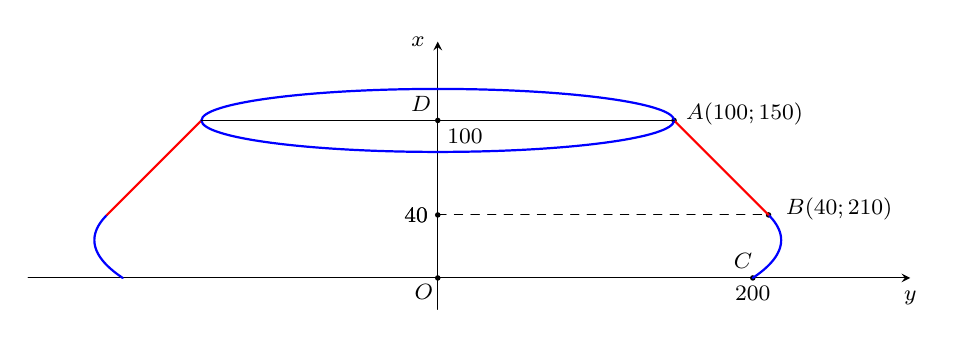
\begin{tikzpicture}[scale=0.02, font=\footnotesize, line join=round, line cap=round, >=stealth]
			\def \xmin{-260}
			\def \xmax{300}
			\def \ymin{-20}
			\def \ymax{150}
			\draw[->] (\xmin,0)--(\xmax,0) node[shift=(-90:0.25)] {$y$};
			\draw[->] (0,\ymin)--(0,\ymax) node[shift=(-180:0.25)] {$x$};
			\fill (0,0) circle(50pt) node[shift=(-135:0.25)]{$O$};
			% ---
			\fill 
			(0,100) circle(50pt) node[shift=(135:0.3)]{$D$} node[shift=(-30:0.4)]{$100$} 
			(200,0) circle(50pt) node[shift=(-90:0.2)]{$200$} node[shift=(120:0.25)]{$C$}
			(150,100) circle(50pt) node[shift=(5:0.9)]{$A(100;150)$}
			(210,40) circle(50pt) node[shift=(5:0.9)]{$B(40;210)$}
			(0,40) circle(50pt) node[left]{$40$}
			;
			\draw[dashed] (0,40) node[left]{$40$} -- (210,40);
			% --- 
			\draw[thick, blue, samples=100, domain=0:40] plot ({-0.03125*(\x)^2 + 1.5*(\x) + 200}, \x);
			\draw[thick, blue, samples=100, domain=0:40] plot ({-(-0.03125*(\x)^2 + 1.5*(\x) + 200)}, \x);
			\draw[thick, red, samples=2, domain=40:100] plot ({-\x + 250}, \x);
			\draw[thick, red, samples=2, domain=40:100] plot ({-(-(\x) + 250)}, \x);
			\draw[thick, blue] (0,100) ellipse (150 and 20);
			\draw[] (150,100) -- (-150,100);
		\end{tikzpicture}
	\end{center}
	\par\shortans[0]{12}
	\loigiai{
		Dựa vào hình vẽ và dữ kiện bài toán, ta xác định phương trình các đường biên của hình phẳng $(H)$
		\begin{itemize}
			\item Gọi phương trình đường thẳng $AB$ có dạng $y=g(x)=ax+b$.\\
			Đường thẳng đi qua hai điểm $A(100;150)$ và $B(40;210)$ nên ta có hệ phương trình
			\[\heva{& 100a+b=150 \\ & 40a+b=210} \Leftrightarrow \heva{& a=-1 \\ & b=250.}\]
			Suy ra phương trình đường thẳng $AB$ là $y=g(x)=-x+250$.
			\item Gọi phương trình parabol $(BC)$ có dạng $y=f(x)=ax^2+bx+c$.\\
			Ta có $f'(x)=2ax+b$.\\
			Parabol đi qua điểm $C(0;200)$, $B(40;210)$ và có tiếp tuyến tại $B$ trùng với đường thẳng $AB$ (có hệ số góc $k=-1$) nên ta có hệ phương trình
			\[\heva{& c=200 \\ & 1\,600a+40b+c=210 \\ & f'(40)=-1} \Leftrightarrow \heva{& c=200 \\ & 1\,600a+40b=10 \\ & 80a+b=-1}
			\Leftrightarrow \heva{& a=-0{,}03125 \\ & b=1{,}5 \\ & c=200.} \]
			Vậy phương trình parabol là $y=f(x)=-0{,}03125x^2+1{,}5x+200$.
		\end{itemize}
		Thể tích của bể bơi là thể tích khối tròn xoay sinh bởi hình phẳng $(H)$ quay quanh trục $Ox$.
		\allowdisplaybreaks
		\begin{align*}
			V &= \pi \displaystyle\int\limits_{0}^{40} [f(x)]^2 \mathrm{\,d}x + \pi \displaystyle\int\limits_{40}^{100} [g(x)]^2 \mathrm{\,d}x \\
			&= \pi \displaystyle\int\limits_{0}^{40} \left(-0{,}03125x^2+1{,}5x+200\right)^2 \mathrm{\,d}x + \pi \displaystyle\int\limits_{40}^{100} (-x+250)^2 \mathrm{\,d}x \\
			&\approx 11\,885\,692{,}21\,\left(\text{cm}^3\right)\\
			&\approx 12 \,\left(\text{m}^3\right).
		\end{align*}
	}
\end{ex}
%%%=============================%%%

%%%=============EX_22=============%%%
\begin{ex}%[2D6C2-4]%[TDMT11]%[Nguyễn Thành Hậu]
	Cho hai hộp, ban đầu hộp I đựng $6$ viên bi đỏ và $4$ viên bi xanh, hộp II đựng $5$ viên bi đỏ và $3$ viên bi xanh, các viên bi có cùng kích thước và khối lượng. Tiến hành lấy ngẫu nhiên $2$ viên bi từ hộp I bỏ sang hộp II. Sau đó, tiến hành lấy ngẫu nhiên từ hộp II ra $3$ viên bi rồi cầm vào tay. Gọi $P$ là xác suất để trên tay có ít nhất một viên bi là của từ hộp I ban đầu, nếu biết các viên bi trên tay đều màu đỏ. Hãy xác định giá trị của $1000P$ (\textit{làm tròn kết quả đến hàng đơn vị}).
	\begin{center}
		\begin{tikzpicture}[scale=0.8,
			bid/.style={circle, draw=red, thick, minimum size=6mm, ball color=red!100, font=\small\bfseries, text=white},
			bix/.style={circle, draw=green, thick, minimum size=6mm, ball color=green!100, font=\small\bfseries, text=white}]			
			%---------------- HỘP I ----------------
			\node at (5,4.6) {\bf HỘP I};
			\draw[thick] (3,4)--(7,4)--(7,1)--(3,1)--cycle;			
			\node[bid] at (6.2,2.46) {};
			\node[bid] at (6.5,1.46) {};
			\node[bid] at (6.14,3.5) {};
			\node[bid] at (4.96,2.36) {};
			\node[bid] at (3.6,2.46) {};
			\node[bid] at (4.5,3.26) {};
			\node[bix] at (3.56,3.46) {};
			\node[bix] at (4.5,1.726) {};
			\node[bix] at (3.56,1.46) {};
			\node[bix] at (5.56,1.46) {};			
			%---------------- HỘP II ----------------
			\node at (11,4.6) {\bf HỘP II};
			\draw[thick] (9,4)--(13,4)--(13,1)--(9,1)--cycle;			
			\node[bix] at (12.04,2.54) {};
			\node[bix] at (9.54,1.54) {};
			\node[bid] at (11.44,1.54) {};
			\node[bid] at (10.48,2.62) {};
			\node[bid] at (9.44,2.46) {};
			\node[bix] at (9.7,3.46) {};
			\node[bid] at (10.88,3.51) {};
			\node[bid] at (12.17,3.6) {};			
		\end{tikzpicture}
	\end{center}
	\par
	\shortans[0]{577}
	\loigiai{
		Gọi $A$ là biến cố \lq\lq Ba viên bi trên tay là màu đỏ\rq\rq.\\
		$B$ là biến cố \lq\lq Trên tay có ít nhất một viên bi của hộp I\rq\rq.\\
		Ta có $\mathrm{P}\left(B\mid A\right)+\mathrm{P}\left(\overline{B}\mid A\right)=1\Rightarrow \mathrm{P}\left(B\mid A\right)=1-\mathrm{P}\left(\overline{B}\mid A\right)=1-\dfrac{\mathrm{P}\left(A\mid\overline{B}\right)\cdot\mathrm{P}\left(\overline{B}\right)}{\mathrm{P}\left(A\right)}$.\\
		Với mỗi $i=0$, $1$, $2$, gọi $T_{i}$ là biến cố \lq\lq Trong hai quả lấy từ hộp I có đúng $i$ quả màu đỏ\rq\rq.\\
		Ta có $\mathrm{P}(A)=\mathrm{P}(AT_{0})+\mathrm{P}(AT_{1})+\mathrm{P}(AT_{2})$.\\
		Ta thấy nếu hai quả lấy từ hộp I không có quả nào đỏ ($2$ quả lấy được là màu xanh) thì hộp II có $5$ viên bi đỏ và $5$ viên bi xanh \[\mathrm{P}(AT_{0})=\dfrac{\mathrm{C}_{4}^{2}}{\mathrm{C}_{10}^{2}}\cdot \dfrac{\mathrm{C}_{5}^{3}}{\mathrm{C}_{10}^{3}}=\dfrac{1}{90}.\]
		Tương tự, $\mathrm{P}\left(AT_{1}\right)=\dfrac{\mathrm{C}_{6}^{1}\cdot\mathrm{C}_{4}^{1}}{\mathrm{C}_{10}^{2}}\cdot \dfrac{\mathrm{C}_{6}^{3}}{\mathrm{C}_{10}^{3}}=\dfrac{4}{45}$, $\mathrm{P}\left(AT_{2}\right)=\dfrac{\mathrm{C}_{6}^{2}}{\mathrm{C}_{10}^{2}}\cdot \dfrac{\mathrm{C}_{7}^{3}}{\mathrm{C}_{10}^{3}}=\dfrac{7}{72}$. Khi đó, \[\mathrm{P}\left(A\right)=\mathrm{P}\left(AT_{0}\right)+\mathrm{P}\left(AT_{1}\right)+\mathrm{P}\left(AT_{2}\right)=\dfrac{1}{90}+\dfrac{4}{45}+\dfrac{7}{72}=\dfrac{71}{360}.\]
		Ta có $\mathrm{P}\left(\overline{B}\right)$ là xác suất mà $3$ viên bi trên tay, lấy từ hộp II mà không có viên bi nào của hộp I nên không phụ thuộc vào việc lấy bi màu gì ở hộp I, do đó $\mathrm{P}\left(\overline{B}\right)=\dfrac{\mathrm{C}_{8}^{3}}{\mathrm{C}_{10}^{3}}=\dfrac{7}{15}$.\\
		Ta có $\mathrm{P}\left(A\mid \overline{B}\right)$ là xác suất mà $3$ viên bi trên tay đều là màu đỏ khi đã biết trên tay không có viên bi nào được lấy từ hộp I (xác suất này cũng không phụ thuộc vào việc lấy bi màu gì ở hộp I) nên $\mathrm{P}\left(A\mid \overline{B}\right)=\dfrac{\mathrm{C}_{5}^{3}}{\mathrm{C}_{8}^{3}}=\dfrac{5}{28}$.\\
		Khi đó, \[\mathrm{P}\left(B\mid A\right)=1-\mathrm{P}\left(\overline{B}\mid A\right) =1-\dfrac{\mathrm{P}\left(A\mid \overline{B}\right)\cdot\mathrm{P}\left(\overline{B}\right)}{\mathrm{P}\left(A\right)}=1-\dfrac{\dfrac{5}{28}\cdot \dfrac{7}{15}}{\dfrac{71}{360}}=\dfrac{41}{71}.\]
		Vậy $1000P=1000\mathrm{P}\left(B\mid A\right)=1000\cdot\dfrac{41}{71}\approx 577$.
	}
\end{ex}
%%%=============================%%%
\Closesolutionfile{ans}
\newpage
\indapan{12}{ans/ansTN-Dung}
\indapan[TF]{2}{ans/ansTN-DungSai}
\indapan[SA]{6}{ans/ansTN-DienKhuyet}
%%%%%%%%%%%%%%
%%nhãn kết thúc đề (để đếm số trang tự động mỗi đề)
\label{B\thedeso}